\section{Testing and Experimentation}\label{sec:testing-and-experimentation}

\subsection{Testing and Experiment Approach}\label{subsec:testing-and-experiment-approach}

\subsubsection{Hardware}

Testing the hardware was an iterative process that entailed using simulations, continuity
checks, and constant soldering of different parts in different ways to conserve space to make
the hardware as physically unobtrusive as possible while keeping it easy to repair. In the
ideation phase, simulations played a pivotal role in assessing different power
deliveries and wiring configurations. The Fritzing software facilitated virtual simulations,
guiding the exploration of different configurations and leading to some of the compromises
made as previously described in
\textbf{Design Constraints, Problems, Trade-offs, and Solutions}. Moving into the assembly
phase, a breadboard was used to test test without spending time and effort repeatedly
soldering and desoldering the configuration. Once the hardware configuration reached a
satisfactory level of performance, only then were the parts soldered together. The prototyping
phase introduced further refinement wherein different wires and connectors were used to
determine the best manner of mounting different components to one continuous connection. A
proof of concept was made that had no consideration for conservation of space, and continuity
checks were done with a multimeter to ensure that each solder connection was made properly.

As the hardware configuration approached finalization, several spare parts were soldered
together and connected onto the board that used different techniques to conserve space. Again,
the solder joints were tested for continuity with a multimeter. Overall, the hardware
development process involved deliberate iterative designs from virtual simulation to physical
prototype, and ease of repair was taken into account by documenting the nature of the solder
joints so end users could easily replicate the consolidation done by the hardware system
integrators.

\subsubsection{Software}

The primary objective of testing the software was to evaluate the functionality, reliability,
and performance of the system across various components and integrations. The testing process
was comprehensive, covering both unit and integration levels to ensure the individual
function of components as well as their cohesion across the system. The initial phase of unit
testing involved exploring the edge cases of each system component in isolation, scrutinizing
the functions and methods within Flask and ReactJS respectively. Special attention was given
to the database interactions and the dependable data transmission between the microcontroller
and the backend server. Subsequently, integration testing was executed to affirm a stable link
between different layers of the system design, to guarantee consistency and accuracy of data.
The efficiency of communication between the microcontroller, sensors, and backend server were
rigorously validated.

\subsection{Testing and Experiment Results and Analysis}\label{subsec:testing-and-experiment-results-and-analysis}

While the majority of test cases passed successfully, demonstrating system
robustness and reliability, any failed tests were promptly addressed,
with bugs fixed and tests rerun until success was achieved. With respect to performance testing, the system performed well under normal simulated conditions as outined in the linked GitHub repository. \cite{MorteSense-2023} In terms of test coverage, new cases were made based on observations from field testing as well as end user testing. To organize and achieve a satisfactory level of test coverage, bugs were categorized based on severity and given a priority level with the help of tools such as GitHub issues.

\begin{figure}[htbp]
      \centering
      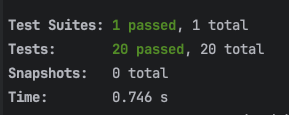
\includegraphics[width=1\linewidth]{datasets/images/Jest-Test-Suite.png}
      \caption{Using Jest Test Suite}
      \label{fig:figure2}

\end{figure}

\begin{figure}[htbp]
      \centering
      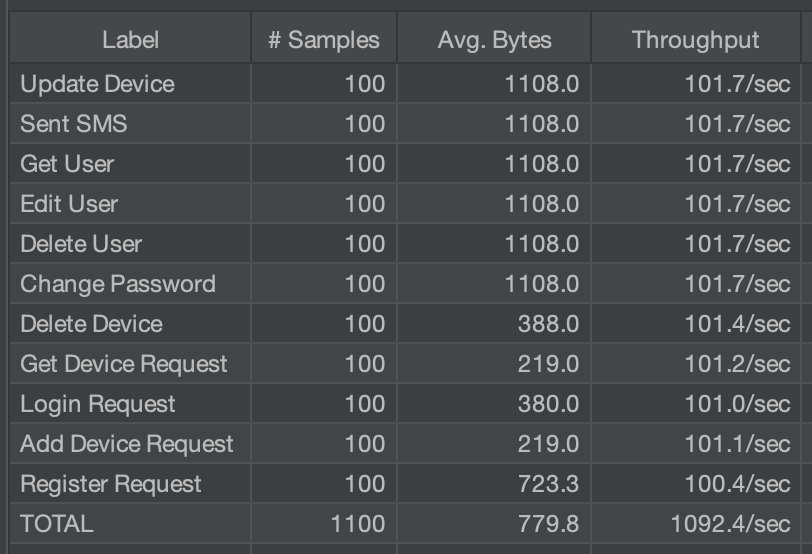
\includegraphics[width=1\linewidth]{datasets/images/JMeter_100reqBenchmark.png}
      \caption{JMeter 100 Request Benchmark Metrics}
      \label{fig:figure3}
\end{figure}

\begin{figure}[htbp]
      \centering
      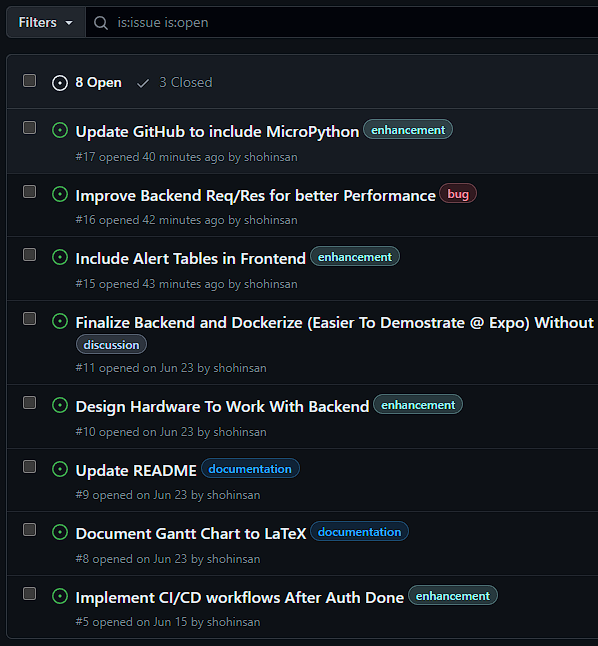
\includegraphics[width=1\linewidth]{datasets/images/GitHubIssues.png}
      \caption{Issue Tracking System}
      \label{fig:gitIssues}
\end{figure}

By rigorously following this comprehensive testing and experiment
approach, the developers ensured that the system was reliable,
performed well, and met all the defined requirements and benchmarks.